% %%%%%%%%%%%%%%%%%%%%%%%%%%%%%%%%%%%%%%%%%%%%%%%%%%%%%%%%%%%%%%%%%%%%%%%%%%%%%
\chapter{Neural Machine Translation}
\label{chap:nmt}
% %%%%%%%%%%%%%%%%%%%%%%%%%%%%%%%%%%%%%%%%%%%%%%%%%%%%%%%%%%%%%%%%%%%%%%%%%%%%%

\Ac{nmt} is the current state-of-the-art approach to \ac{mt}. As the name
suggests, the underlying machine learning concept in \ac{nmt} systems are
neural networks. The specific types, or \emph{architectures}, of neural
networks used in an \ac{nmt} system vary across history, applications, or
domains, but all share a few common traits.

Neural networks are a mathematical model that works with real numbers: The
inputs and the outputs to a neural network are real-valued vectors, the
training objective is a differentiable function, and the space of the
parameters needs to have a continuous gradient with respect to the loss
function. Specific to neural networks is the computation of the gradient by the
\emph{backpropagation} algorithm, and the large portfolio of optimization
methods.

In Section \ref{sec:text-processing}, we explain how to adapt neural networks
to the discrete nature of the textual data. Perhaps the most common way is to
assign a real-valued vector to each word in the vocabulary. These
representations are usually trained along with the whole network, end to end.

In \acs{nlp} tasks like sentence classification or language modeling, there is
only a single sequence on the input. In \ac{mt}, we have a source sentence on
the input, and a target sentence on the output. To reflect this property, most
of the \ac{nmt} architectures have two components: an \emph{encoder} and a
\emph{decoder}. The encoder processes the input sentence and creates a hidden
representation. The decoder then accesses this hidden representation and
generates (or scores) the output sentence. When both components of the model
are trained end to end, this framework is sometimes referred to as
\emph{sequence-to-sequence learning}. We explore the encoder-decoder
architectures more closely in Section \ref{sec:encdec}.

Textual data are sequential and the lengths of the sequences are
variable. Using feed-forward neural networks is therefore not
suitable. Sequences can be processed by a number of network architectures,
namely \acp{cnn}, \acp{rnn}, or \acp{san}. All of those can be adapted for text
processing, and we will describe the latter two in more detail in Sections
\ref{sec:encdec:rnn} and \ref{sec:encdec:transformer}, respectively.

% Section about training: batching, optimization, multiple GPUs, ...
\ac{nmt} models are trained using large parallel corpora, by minimizing the
negative log-likelihood of the data.  Section \ref{sec:training} formalizes the
supervised training framework for translation models and summarizes the
training methodology, such as data processing, model initialization, and
optimization.

% Section about decoding
During training, sequence-to-sequence decoders usually run in the \emph{teacher
  forcing} mode -- for a given source sentence and its translation, the neural
network is trained to maximize the likelihood of $i$-th target word on $i$-th
position, conditioned on the $i-1$ previous words of the reference
sentence. During decoding, when this information is not available, the model is
conditioned on previously decoded outputs instead. More details on this
phenomenon and other practical considerations and techniques such as beam
search or ensembling are presented in Section \ref{sec:decoding}.

% alternative paragraph for Training section overview. Focus on batching and
% optimization instead of teacher forcing.

\Ac{mt} is evaluated by automatic metrics such as \acs{bleu} and by human
evaluation. This chapter concludes with a brief overview of the evaluation of
\ac{nmt} systems (Section \ref{sec:evaluation}).

% ------------------------------------------------------------------------------
\section{Processing Text with Neural Networks}
\label{sec:text-processing}
% ------------------------------------------------------------------------------

% Text are not numbers, NNs work with numbers
There are a number of problems that arise when we want to use neural networks
for text processing. Foremost, neural networks are a mathematical model that
deals with real numbers. In contrast, language is discreet and has a complex
structure. Thus, we need to find ways of expressing textual data
numerically. Second, since language units (such as words, sentences, or
documents) come in various lengths, we need to use neural network models
designed for processing sequential data.

% One-hot representation are straightforward.
In this section, we begin with the representation of words. The most
straightforward, and also the most common way to represent words in neural
networks is by having a list (a \emph{vocabulary}) of words $\mathcal{V}$, where each
word has a corresponding integer index $j$ pointing at it. Each word $w$ at
index $j$ in this list can be represented by a vector
$x \in \{0,1\}^N$ where
%
\begin{equation} x_i =
\begin{cases} 1, & \text{if } i = j \\ 0, & \text{otherwise.}
\end{cases}
\end{equation}
%
We call this vector the \emph{one-hot representation} of $w$.

% One-hot representation do not capture word roles in language.
Using one-hot representation help us convert discreet words to numbers, but it
does not capture anything about the underlying linguistic structure.  For this
purpose, \emph{learned distributed feature vectors}, or \emph{word embeddings}
are used \citep{bengio2003neural, collobert-weston-2007-fast}. The idea is to
associate a real-valued vector with each word, so that representations of words
with similar roles in language are closer together in the assigned vector
space. \citet{mikolov-etal-2013-distributed} train these word embeddings using
the \emph{skip-gram} and \emph{continuous bag of words} objectives and find
that the resulting embeddings have interesting properties. For example,
arithmetic operations on embeddings can express word analogy.  In some \ac{nlp}
tasks, pre-trained embeddings can be used to greatly improve the model
performance on the end task. In contemporary \ac{nmt} research, the most
prevalent approach is to train the word embeddings end-to-end along with the
translation model.

% Word embedding layer is inserted to help.
We provide the model with the distributed representation of words using an
embedding layer as follows. For a given one-hot vector $x$, and a
parameter matrix $E$ called the \emph{embedding matrix}, we retrieve a single
row that corresponds to the vocabulary index of $x$ by the
multiplication $E x$.
% %
% \begin{equation}
%   e(\mathbf{w}) = E\mathbf{w}.
% \end{equation}
% %
The embedding dimension is usually much lower than the size of the vocabulary
(in \ac{nmt}, the embedding dimension in state-of-the-art models is around
1,024).

% There are out-of-vocabulary tokens
A major drawback of having a fixed-size vocabulary is the fact that there will
be unseen words in the data. The following section lists methods that solve
this problem.

\subsection{Open Vocabulary Problem}

% Zipf nature of language
A well known characteristic of language is that it follows the Zipf's law
\citep{zipf1949human}. As a result, in a large enough sample of text, there is
a huge amount of unique words or words occurring with low frequency. Such words
constitute a substantial part of the data and cannot be ignored.  Another issue
is that our training datasets do not contain all words that can occur in the
language. These \ac{oov} words usually also make up significant portions of the
validation and test data.

% Open vocabulary problem
The problem of rare and unseen words is also referred to as the \emph{open
  vocabulary} problem. Although some work in this direction exist
\citep{jean-etal-2015-using}, in neural networks for \ac{nlp}, it is difficult
to use very large vocabularies. The main reason is that the embedding layer and
the output projection layer would become too large for the computation to be
efficient.

% Most common solution
The most common solution of the open vocabulary problem is to use smaller units
than words \citep{sennrich-etal-2016-neural}. These \emph{subword} units can be
constructed in a smart way, such that frequent words are left intact, whereas
rare words are composed of more common strings of letters. Below, we describe
three of the methods for subword segmentation. It is worth mentioning that the
research on character-level methods is still ongoing, but as of the writing of
this thesis, this approach did not yet outperform the subword state-of-the-art
\citep{chung-etal-2016-character,lee-etal-2017-fully,gao-etal-2020-character}.

% - - - - - - - - - - - - - - - - - - - - - - - - - - - - - - - - - - - - - - -
\paragraph{\acs{bpe}.}  \Acl{bpe} \glsunset{bpe} (\acs{bpe};
\citealp{sennrich-etal-2016-neural}) is an approach which tackles the open
vocabulary problem by splitting words to subword units.  The idea is to devise
a vocabulary of a predefined size, such that any word can be composed using the
units from the vocabulary (with the exception of words containing unknown
characters). An additional requirement is for the vocabulary to contain whole
words which are frequent in the data, so only rare words are split into more
subwords. The \ac{bpe} method works with a vocabulary of merges, which needs to
be created by the \ac{bpe} training algorithm before it can be applied on the
data.

The \ac{bpe} training algorithm proceeds in iterations as follows. In the
beginning, all tokens in the data are split into characters, and the vocabulary
is initialized with the list of the characters. To allow for later
reconstruction of the original text, a special end-of-word character is
appended to each word.  Each iteration of the algorithm has three steps. First,
the algorithm computes the counts of pairs of consecutive symbols (bigrams) in
the data (respecting the word boundaries), and selects the most frequent
pair. Second, the selected bigram is merged and added to the vocabulary. Third,
the new vocabulary is used to segment the data again. These three steps are
repeated until a predefined number of merges is performed.  Note that in
practice, the algorithm can be implemented to work only with the frequency list
of tokens, and not with the whole training corpus, without loss of generality.

Once the \ac{bpe} merge list is created, it can be applied on the data by first
splitting the words in the data to characters, and then applying the learned
merges on the split words. Reconstruction of the original text can be done by
removing the spaces and then replacing the end-of-word characters with new
spaces.

% - - - - - - - - - - - - - - - - - - - - - - - - - - - - - - - - - - - - - - -
\paragraph{Wordpiece.} The wordpiece algorithm
\citep{schuster-nakajima-2012-japanese,wu2016google} shares the ideas of the
\ac{bpe} algorithm -- whole words are split into sequences of characters, which
are then merged according to a list of merges. Unlike the \ac{bpe}
segmentation, the wordpiece learning algorithm does not take the most frequent
bigram, but instead the pair with the biggest pointwise mutual
information. \JH{They say they take the pair that maximizes the likelihood of
  the data, but then we would need to talk about language models first, and I
  guess it's the same thing.}


% - - - - - - - - - - - - - - - - - - - - - - - - - - - - - - - - - - - - - - -
\paragraph{SentencePiece.} More recently,
\citet{kudo-richardson-2018-sentencepiece} implemented Sentencepiece, a toolkit
for subword segmentation using either \ac{bpe}, or a unigram language model
\citep{kudo-2018-subword}. It supports a number of features, such as sampling
and regularization by introducing noise on the source side. As opposed to BPEs
and wordpieces, Sentencepiece does not require prior tokenization of the input
text, and unlike other methods its pre-tokenization allows to fully reconstruct
the original string. The Marian toolkit
\citep{junczys-dowmunt-etal-2018-marian} used in our experiments described in
Chapter \ref{chap:experiments} has a built-in support for Sentencepiece
tokenization and segmentation.

% ------------------------------------------------------------------------------
\section{Encoder-Decoder Framework}
\label{sec:encdec}
% ------------------------------------------------------------------------------

The contemporary \ac{nmt} models share a common framework where each model is
composed of two parts -- an \emph{encoder}, and a \emph{decoder}. The encoder
reads in the input sentence and processes it in order to generate an
intermediate hidden representation.  The decoder then uses this intermediate
hidden representation to produce the probability distributions over the output
tokens.

The early \ac{nmt} models based on \acp{rnn} use the final encoder state as the
intermediate representation \citep{sutskever2014sequence}:
%
\begin{align}
  h_j &= \mathrm{RNN}_{\text{enc}}(x_j, h_{j-1}), \quad j \in
          \{0, 1, \ldots, T_x \} \\
  s_0 &= h_{T_x}
\end{align}
%
where $\mathbf{x}$ is the input sentence and $h_0$ is the initial hidden state,
usually set to $\mathbf{0}$. $T_x$ denotes the length of the input sentence.
Note that the input words are represented as their embeddings.
\citet{sutskever2014sequence} do not use subword segmentation and instead
reserve a special OOV token for unseen words.

The decoder is initialized with the state $s_0$ and runs the second \ac{rnn}:
\begin{equation} s_i = \mathrm{RNN}_{\text{dec}}(y_{i-1}, s_{i-1})
\end{equation}
%
where $y_{i-1}$ is the preceding word in the reference output sentence (during
training), with $s_0$ being a special symbol which expresses the start of a
sequence (denoted \texttt{<s>}).

While recurrent neural networks are not used as the underlying model in the most
of the current research anymore, the encoder-decoder framework is independent of
the actual neural network structure and the concept is still used as a main
approach for designing sequence-to-sequence models.

In this section, we introduce the two most notable encoder-decoder
architectures. The first is based on \acp{rnn} and became the first neural
architecture to outperform statistical \ac{mt} models. The second architecture,
called \emph{Transformer}, is based on self-attentive networks and is the
best-performing architecture for many \ac{nlp} tasks today.


% - - - - - - - - - - - - - - - - - - - - - - - - - - - - - - - - - - - - - - -
\subsection{Recurrent Neural Networks}
\label{sec:encdec:rnn}
% - - - - - - - - - - - - - - - - - - - - - - - - - - - - - - - - - - - - - - -

The invention of \acp{rnn} \citep{elman1990finding} allowed processing of
sequential data by neural networks. \Acp{rnn} process the sequence one item at
a time, chaining consecutive steps with recurrence connections.

In the early stages of the \ac{rnn} development, a single hidden layer of the
network was altered to take into account the output of itself from the previous
time step:

%\begin{equation} % h_t = f(x_t, h_{t-1})
%\end{equation}
%
%\noindent %where $f$ is usually a non-linear projection:

\begin{equation} h_t = \tanh ( W x_t + U h_{t-1} + b_h ) \label{eq:vanilla-rnn}
\end{equation}

\noindent where $W \in \mathbb{R}^{m \times n}$,
$U \in \mathbb{R}^{n \times n}$, $b_h \in \mathbb{R}^{n}$ are trainable
parameters, $x_t \in \mathbb{R}^{m}$ is the \ac{rnn} input, and
$h_{t-1} \in \mathbb{R}^{n}$ is the previous hidden state.

This version of \acp{rnn} however suffers from the \emph{vanishing gradient
  problem}. During backpropagation, the gradients are multiplied with the
derivative of the hyperbolic tangent, which is always less or equal to one. In
long sequences, the learning signal over distant parts of the sequence has
therefore almost no effect on the training. Due to this fact, the network
manifests poor performance in handling long-range dependencies.

There has been several approaches to combat the vanishing gradient problem.
The most prevailing types of \ac{rnn} architectures in \ac{nmt} are \ac{lstm}
networks and \ac{gru} networks.

% - - - - - - - - - - - - - - - - - - - - - - - - - - - - - - - - - - - - - - -
\paragraph{\acs{lstm}.} \acl{lstm} networks \citep{hochreiter1997long}
introduce gating mechanisms and a concept of \emph{information highway}, which
ensures that only linear operations are applied on the states in the recurrent
chain. A gating mechanism is an operation which computes a number between 0 and
1, which we refer to as \emph{gate value}.  The output of the operation is the
input multiplied by the gate value.

Given a current time step $t$, input $x_t \in \mathbb{R}^m$, and previous
hidden states $h_{t-1}, C_{t-1} \in \mathbb{R}^n$, \ac{lstm} networks proceed
as follows:
%
\begin{align}
  f_t &= \sigma\left(W_f x_t + U_f h_{t-1} + b_f\right) \label{eq:lstm-forget-gate} \\
  i_t &= \sigma\left(W_i x_t + U_i h_{t-1} + b_i\right) \label{eq:lstm-input-gate} \\
  o_t &= \sigma\left(W_o x_t + U_o h_{t-1} + b_o\right) \label{eq:lstm-output-gate} \\
  \tilde{C}_t &= \tanh \left( W_c x_t + U_c h_{t-1} + b_c \right) \label{eq:lstm-candidate} \\
  C_t &= f_t \odot C_{t-1} + i_t \odot \tilde{C}_t \label{eq:lstm-information-highway} \\
  h_t &= o_t \odot \tanh C_t \label{eq:lstm-hidden-state}
\end{align}
%
where $W_f, W_i, W_o, W_c \in \mathbb{R}^{m \times n}, U_f, U_i, U_o, U_c \in
\mathbb{R}^{n \times n}, b_f, b_i, b_o, b_c \in \mathbb{R}^n$ are trainable
parameters, $\sigma$ is the logistic function, and $\odot$ represents
element-wise multiplication. The states $h_t$ and $C_t$ are also called public
and private hidden states respectively. The intermediate value $\tilde{C}_t$ is
called the candidate state.

The three gates in the \ac{lstm} network are called \emph{forget gate},
\emph{input gate}, and \emph{output gate}. The forget gate (Eq.
\ref{eq:lstm-forget-gate}) controls how much of the information from the
previous private hidden state $C_{t-1}$ to the current private state (Eq.
\ref{eq:lstm-information-highway}). The input gate (Eq.
\ref{eq:lstm-input-gate}) controls the amount of information received from the
candidate state. Finally, the output gate (Eq. \ref{eq:lstm-output-gate})
decides which portion of the currently computed private hidden state is
transferred to the current public hidden state
(Eq. \ref{eq:lstm-output-gate}). Note that the values of the gates are computed
in the same way, but with different parameters.

The original recurrence relation from Equation \ref{eq:vanilla-rnn} is expressed
by Equation \ref{eq:lstm-candidate}, where the new candidate state is
computed. The transfer of information from the previous private state and the
current candidate state is done in Equation
\ref{eq:lstm-information-highway}. Note that with respect to the states from the
preceding steps, the previous state is only multiplied by a constant. This
constitutes the information highway that allows propagating the gradients over
long distances in the sequence.

% - - - - - - - - - - - - - - - - - - - - - - - - - - - - - - - - - - - - - - -
\paragraph{\acs{gru}.} \acl{gru} networks \citep{cho2014gru} are an alternative
to \acp{lstm}. Instead of four sets of parameter matrices, \acp{gru} need only
three, while maintaining the theoretical strength. Unlike \acp{lstm}, \acp{gru}
use only a single hidden state in the recurrence relations.

Given the time step $t$, input $x_t \in \mathbb{R}^m$, and previous hidden
state $h_{t-1}$, one \ac{gru} step is defined as follows:
%
\begin{align}
  r_t &= \sigma\left(W_r x_t + U_r h_{t-1} + b_r\right) \label{eq:gru-reset-gate} \\
  z_t &= \sigma\left(W_z x_t + U_z h_{t-1} + b_z\right) \label{eq:gru-update-gate} \\
  \tilde{h}_t &= \tanh \left(W x_t + U \left( r_t \odot h_{t-1} \right) + b \right) \label{eq:gru-candidate} \\
  h_t &= (1 - z_t) \odot h_{t-1} + z_t \odot \tilde{h}_t \label{eq:gru-hidden-state}
\end{align}
%
where $W, W_z, W_r \in \mathbb{R}^{m\times n}$,
$U, U_z, U_r \in \mathbb{R}^{n \times n}$, and $b, b_z, b_r \in \mathbb{R}^n$
are trainable parameters.

The two gates in \ac{gru} networks are called \emph{reset gate} and
\emph{update gate}.  The reset gate (Eq. \ref{eq:gru-reset-gate}) determines
how much of the information from the previous state is preserved and is applied
in the recurrence relation for computing the candidate
(Eq. \ref{eq:gru-candidate}). The update gate (Eq.  \ref{eq:gru-update-gate})
controls the merging of the previous state with the candidate state in Equation
\ref{eq:gru-hidden-state}. Note that the information highway concept is
expressed by this equation.

% - - - - - - - - - - - - - - - - - - - - - - - - - - - - - - - - - - - - - - -
\paragraph{Bidirectional RNNs.} There is a bidirectional variant of \acp{rnn}
which can be applied to any of the flavors of \acp{rnn} discussed above. When
the whole input sequence is known, we can apply a \ac{rnn} in both directions
separately and then concatenate the states from the corresponding positions:
%
\begin{align}
  \overrightarrow{h}_t &= \overrightarrow{\mathrm{RNN}}(x_{t-1}, \overrightarrow{h}_{t-1}) \\
  \overleftarrow{h}_t &= \overleftarrow{\mathrm{RNN}}(x_{t+1}, \overleftarrow{h}_{t+1}) \\
  h_t &= \left[ \begin{matrix} \overrightarrow{h}_t \\ \overleftarrow{h}_t \end{matrix} \right]
\end{align}

% - - - - - - - - - - - - - - - - - - - - - - - - - - - - - - - - - - - - - - -
\paragraph{Attention Mechanism.} Another important concept introduced as a part
of \ac{rnn}-based \ac{nmt} models is the \emph{attention mechanism}
\citep{bahdanau2014neural,luong-etal-2015-effective}.

The problem with the encoder-decoder framework as described in the previous
section is that there is an information bottleneck between the encoder and the
decoder. All the information from the source sentence needs to be compressed
into a single hidden state vector $s_0$.

The attention mechanism enables the decoder to access the information stored in
the encoder hidden states rather than relying only on the value of the initial
state.  Formally, based on a current decoder step $s_i$, the attention mechanism
computes a local \emph{context vector} as a weighted average of the encoder
states:
%
\begin{align}
  % attn energies
  e_{ij} &= v_a^\top \tanh (W_a s_{i-1} + U_a h_j + b_a) + b', \label{eq:attn-energies} \\
  % attn distro
  \alpha_{ij} &= \frac{\exp(e_{ij})}{\sum_{k=1}^{T_x}\exp(e_{ik})}, \\
  %
  % \softmax_{j \in 1, 2, \ldots, T_x } & = & e_{ij} \\
  % context vector
  c_i &= \sum_{j=1}^{T_x} \alpha_{ij} h_j.
\end{align}
%
In the first step, the \emph{attention energies} are computed for every encoder
hidden state using a single-hidden-layer feed-forward network parameterized by
$W_a \in \mathbb{R}^{n' \times n}$, $U_a \in \mathbb{R}^{n' \times 2n}$,
$b_a \in \mathbb{R}^{n'}$, $v_a \in \mathbb{R}^{n'}$, and $b' \in \mathbb{R}$
where $n'$ is the dimension of the hidden layer. Next, the attention energies
are normalized using the softmax function into the \emph{attention
  distribution}.  Finally, the context vector is computed as a weighted sum of
the encoder states $h_0,\ldots, h_{T_x}$, using the attention distribution
values as weights.

The concept of attention can be viewed as a soft-lookup function over an
associative memory. Given a \emph{query}, which is the decoder state in a given
time step, we use a similarity metric over a set of \emph{keys}. We then
normalize the similarities and use them as weights in the weighted sum of
\emph{values} associated with the corresponding keys. In this case, the sets of
attention keys and values are equal -- the encoder hidden states $h_j$. The
similarity metric is defined in Equation \ref{eq:attn-energies}.

% - - - - - - - - - - - - - - - - - - - - - - - - - - - - - - - - - - - - - - -
\paragraph{Deep \acp{rnn}.} Some NMT architectures based on RNNs use multiple
recurrent layers \citep{barone2017deep,wu2016google}. In deep RNNs, each layer
is a recurrent network. The inputs of the second and each layer onwards are the
outputs of the preceding layer. The output of the whole deep RNN is the output
of the last layer.

In deep \acp{rnn}, there are a few settings to consider. \JH{tell me more}

\JH{first layer norm paragraph should give better motivation, last paragraph
  should provide some insight to the formulas.}  To improve the convergence
speed of the deep models, \emph{layer normalization} \citep{ba2016layer} is
often employed between layers. For layer $l$ and its output states
%$h_1^l, \ldots h_{T_x}^l$, $h_i^l \in \mathbb{R}^n$,
$\mathbf{h}^l \in \mathbb{R}^{T_x \times n}$, we compute:
%
\begin{align}
  \mu^l &= \frac{1}{nT_x} \sum_{i=1}^{T_x}\sum_{j=1}^n h^l_{ij} \\
  \sigma^l &= \sqrt{\frac{1}{nT_x} \sum_{i=1}^{T_x}\sum_{j=1}^n (h^l_{ij} - \mu^l)^2} \\
  \bar{\mathbf{h}}^l &= \frac{\mathbf{h}^l - \mu^l}{\sigma^l} \odot \gamma^l + \beta^l
\end{align}
%
where $\mu^l$ and $\sigma^l$ are the mean and standard deviation of the output
state values, $\gamma^l, \beta^l \in \mathbb{R}^{T_x \times n}$ are learnable
\emph{gain} and \emph{bias} parameters, and $\odot$ denotes element-wise
multiplication. The normalized states $\bar{\mathbf{h}}^l$ are then used as the
input to the $l+1$-th layer of the network instead.




% - - - - - - - - - - - - - - - - - - - - - - - - - - - - - - - - - - - - - - -
\subsection{Transformer Model}
\label{sec:encdec:transformer}
% - - - - - - - - - - - - - - - - - - - - - - - - - - - - - - - - - - - - - - -

One of the disadvantages of the RNN-based models is the sequential nature of
the recurrence relation. Few models have been proposed to remove the recurrence
and thus allowing for simultaneous computation across time steps, at least at
the training time. Most notably, these models include convolutional
architectures \citep{gehring2017convolutional}, and the current
state-of-the-art architecture, the \emph{Transformer} model
\citep{vaswani2017attention}.

Instead of recurrence relations, the Transformer model uses
\emph{self-attention} layers, stacked into a deep network. The states in each
layer can be computed independently on each other, which makes room for
training speed improvements. We follow with detailed description of the
Transformer model components. Refer to Figure \ref{fig:transformer} for
the overview of the model components.

\begin{figure}
  \centering
  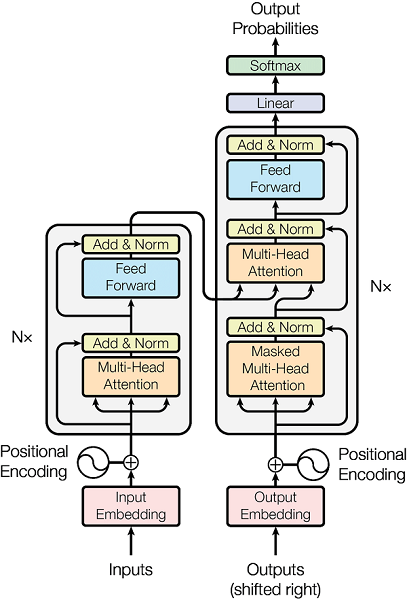
\includegraphics[width=9cm]{img/transformer.png}

  \caption{The overall schema of the Transformer model. Inputs are summed with
    positional encodings. Encoder processes the input in $N$ stack layers. Each
    encoder layer consists of self-attention and feed-forward sub-layer. Layers
    are interconnected with residual connections and layer normalization is
    applied on the output of each layer. The decoder stack uses three
    sub-layers, where the additional cross-attention layer attends to the
    encoder output. We show the original image from
    \citet{vaswani2017attention}.}
  \label{fig:transformer}
\end{figure}

% - - - - - - - - - - - - - - - - - - - - - - - - - - - - - - - - - - - - - - -
\paragraph{Positional Encoding.} Since the self attention is a commutative
operation, the ordering of the input tokens needs to be modeled explicitly.
The standard technique is to use sinusoidal encodings, proposed in the original
paper. Positional encoding is a vector of the same dimension as the word
embedding which is computed using the position of the word on the input.
The $2i$-th and $(2i+1)$-th elements of the positional encoding of word on
position $j$ is computed as follows:
%
\begin{equation}
  \begin{split}
    E_{\text{pos}}(j, 2i) &= \sin(j / 10000^{2i/d}) \\
    E_{\text{pos}}(j, 2i + 1) &= \cos(j / 10000^{2i/d})
  \end{split}
\end{equation}
%
where $d$ is the \emph{model dimension}. This number is equal to the dimension
of the word embeddings. Before an input word $w_i$ is processed by the network,
the positional encodings are added to the word embeddings:
\begin{equation}
  E(w_i) = E(w) + E_{\text{pos}}(i)
\end{equation}

% - - - - - - - - - - - - - - - - - - - - - - - - - - - - - - - - - - - - - - -
\paragraph{Self-Attention.} The key component of the Transformer model is the
self-attention. As the name suggests, self-attention is run with the same set
of states used as both queries, keys, and values. Scaled dot-product is used as
the similarity metric, so the attention itself does not use any trainable
parameters. Formally, self-attention is defined as function:
%
\begin{equation}
  \mathcal{A}(Q,K,V) = \softmax \left( \frac{QK^\top}{\sqrt{d}} V  \right)
  \label{eq:scaled-dot-product}
\end{equation}
%
where the values $Q, K, V \in \mathbb{R}^{T \times d}$ ($T$ being the sequence
length) are computed from the same input, usually using a linear projection.

Self-attention sub-layers are used both in the encoder and the decoder. Because
the decoder is autoregressive, the self-attention module needs to be
constrained to attend only to the preceding states (so the model does not
``glance into the future''). This is implemented by applying a triangular mask
(also \emph{causal mask}) on the attention query and key matrix, hence the name
\emph{masked self-attetnion}.

% - - - - - - - - - - - - - - - - - - - - - - - - - - - - - - - - - - - - - - -
\paragraph{Multi-Head Attention.} Instead of running a single self-attention
per layer, the model structure is enriched by splitting the self-attention into
multiple \emph{heads}. First, each state is projected into $h$ triples of
queries, keys, and values. Then, self-attention is computed on each triple.
Finally, the self attention outputs are mixed together into a single output
sequence:
%
\begin{equation}
  \mathcal{A}^h(Q, K, V) = \sum_{i=1}^h C_i W_i^O \\
\end{equation}
%
where $W_i^O \in \mathbb{R}^{d_h \times d}$ is a parameter matrix used for
projecting the outputs from the individual attention heads into a single
output, and
%
\begin{equation}
  C_i = \mathcal{A}(QW_i^Q, KW_i^K, VW_i^V)
\end{equation}
where $W_i^Q, W_i^K, W_i^V \in \mathbb{R}^{d \times d_h}$ are trainable
matrices that project the states to inputs for the $i$-th attention head
(defined in Equation \ref{eq:scaled-dot-product}). In self-attention,
$Q = K = V \in \mathbb{R}^{T \times d}$ is the set of $T$ states of the current
layer.

% - - - - - - - - - - - - - - - - - - - - - - - - - - - - - - - - - - - - - - -
\paragraph{Cross-Attention.} Each layer in Transformer encoder consists of a
self-attention and a feed-forward sub-layer. The decoder inserts an
\emph{encoder-decoder attetnion}, or \emph{cross-attention} layer.  The
cross-attention layer functions exactly like self-attention layer, but the
queries $Q$ are the decoder states (i.e. the output of the preceding
self-attention), and the keys and values $K = V$ correspond to the encoder
output states.

% - - - - - - - - - - - - - - - - - - - - - - - - - - - - - - - - - - - - - - -
\paragraph{Feed-Forward Layer.} Each Transformer layer consists
of self-attention, optionally a cross-attention, followed by a feed-forward
network. This feed-forward network uses the same parameters for all positions
along the state sequence. The network takes a state $x$ and feeds it through a
single hidden layer with a ReLU activation:

\begin{equation}
  \mathcal{F}(x) = \max(0, W_1^Fx + b_1^F)W_2^F + b_2^F
\end{equation}
where $W_1^F \in \mathbb{R}^{d \times d_f}$, $b_1 \in \mathbb{R}^{d_f}$,
$W_2^F \in \mathbb{R}^{d_f \times d}$, and $b_2^F \in \mathbb{R}^d$ are the
weight and bias parameters of the feed-forward network $\mathcal{F}$, and $d_f$
is the dimension of the hidden state.

% - - - - - - - - - - - - - - - - - - - - - - - - - - - - - - - - - - - - - - -
\paragraph{Residual Connections and Layer Normalization.} As a post-processing
step, the output of each sub-layer is connected with the output of the previous
sub-layer with residual connections. \JH{zkontrolovat jestli se to definovalo v
  Deep Architectures, stejně jako Layer Norm.} Similarly to the \acs{rnn}-based
deep architectures, layer normalization is used in combination, which ties all
states in the sub-layer stack into a shared vector space.

% - - - - - - - - - - - - - - - - - - - - - - - - - - - - - - - - - - - - - - -
\paragraph{Output Projection.} The states from the last decoder layer are
projected to the size of the vocabulary and interpreted as unnormalized
probability distributions over the output tokens. When a probability
distribution is needed (during training or beam search decoding), the scores
are normalized using the softmax function:
%
\begin{equation}
  p(y_t | y_{<t}, x, \theta) = \softmax( W^S s_t + b^S )
\end{equation}
%
where $W^S \in \mathbb{R}^{d \times |\mathcal{V}|}$,
$b \in \mathbb{R}^{|\mathcal{V}|}$ are the output projection parameters and
$s_t$ is the $t$-th state in the last decoder layer, and $\theta$ is the set of
the model parameters. Note that the probability of the $t$-th output token
$y_t$ is conditioned on the preceding tokens $y_{<t}$ because of the causal
mask in the decoder self-attention. In the Transformer model, it is possible to
tie the values of the output projection matrix with the transposed embedding
matrix. This reduces the number of model parameters and can have advantages
over separate input and output projection matrices when using a shared
source--target vocabulary.

To compute the probability distribution of the whole target sentence $y$ given
the input sentence $x$, the distributions from all time steps are multiplied
together:
%
\begin{equation}
  p(y|x) = \prod_{t=1}^{T_y}p(y_t|y_{<t},x,\theta)
  \label{eq:output-distribution}
\end{equation}
%
where $T_y \in \mathbb{R}$ is the length of the target sentence, $y_{<t}$ are
the previously decoded words.

% - - - - - - - - - - - - - - - - - - - - - - - - - - - - - - - - - - - - - - -
\paragraph{Model Hyperparameters.} The parameters that control the model size
are the model dimension $d$, the number of attention heads $h$, the dimension
of the feed-forward hidden layer $d_f$, and the number of Transformer layers in
the encoder and decoder stack. Note that the dimension of keys and values in a
single attention head $d_h$ is commonly set to be $d / h$, but can be
customized as well.  As a regularization, dropout \citep{srivastava2014dropout}
is applied with rate $P_d$ to the output of each sub-layer before
normalization.

The authors of the architecture propose two presets for these parameters, named
\emph{base} and \emph{big}. Table~\ref{tab:transformer-hyperparams} shows the
hyperparameter values for these two settings.

\begin{table}
  \centering
  \begin{tabular}{lrrrrrr}
    \toprule
      & \# of layers &  $d$  &  $h$  & $d_h$ & $d_f$ & $P_d$ \\
    \midrule
    Transformer base  & 6 &  512  & 8 & 64 &  2,048 & 0.1 \\
    Transformer big  & 6 &  1,024  & 16 & 64 &  4,096 & 0.3 \\
    \bottomrule
  \end{tabular}
  \caption{The hyperparameter values for Transformer base and big variants.}%
  \label{tab:transformer-hyperparams}
\end{table}


% ------------------------------------------------------------------------------
\section{Training}
\label{sec:training}
% ------------------------------------------------------------------------------

Training of \ac{nmt} models is usually done under \emph{supervised} conditions,
using a dataset of parallel sentences. \JH{move the following to the
  experimental section:} The size of the available data varies a lot with
different language pairs. Although there is no formal definition, when there is
less than a million sentence pairs available, the language pair is reffered to
as being \emph{low-resource}. For many languages, even a million sentences is a
very large number compared to what is actually available. The data quality is
also a factor. For example, when the only available data is crawled from the
web, data cleaning can filter out a major part of the corpus. In this thesis,
we focus on language pairs where the data size is not a major issue and we
simulate the low-resource scenario using Romanian-English translation.

Translation models are trained by minimizing the loss function, usually
expressed by cross-entropy between the output distribution and the one-hot
distribution which assigns the probability of one to the correct target word,
and zero probabilities to the other words. Assuming $y_i$ is the correct target
word at position $i$, $p_{\text{ref}}$ is the one-hot distribution, and $p$ is
the distribution predicted by the model, we have:
%
\begin{equation}
  \begin{split}
    H(p_{\text{ref}}, p) &=  - \sum_{w \in \mathcal{V}} p_{\text{ref}}(w) \log p(w) = \\
    &=  - \log p(y_i)
  \end{split}
\end{equation}
%
where $\mathcal{V}$ is the vocabulary. Note that in autoregressive models, the
output distributions $p$ and $p_{\text{ref}}$ are conditioned on the preceding
target words.

Given model parameters $\theta$, the word-level cross-entropy is summed across
the sentence pairs in the data $D$ to obtain the negative log likelihood of the
dataset $J(\theta)$:
%
\begin{equation}
  \begin{split}
  J(\theta) &= - \sum_{(x, y) \in D} \sum_{i = 1}^{T_y} \log p(y_i | x, y_{<i}, \theta) \\
  &= - \sum_{(x, y) \in D} \log p(y | x, \theta)
  \end{split} \label{eq:loss}
\end{equation}
%
where $y_{<i}$ denote the target prefix and $T_{y}$ is the length of the target
sentence $y$. The probability of a sentence can be reformulated using the chain
rule.
\JH{rovnice J hvězdička = argmin J over thetas}

% Since the probability distributions are conditioned on the previously decoded
% tokens, the likelihood of the target sentence is reformulated using the chain
% rule:
% %
% \begin{equation}
%   J_{\theta} = - \sum_{(x, y) \in D} \sum_{i = 1}^{T_y} \log p(y_i | x, y_{<i}, \theta)
% \end{equation}
% %
% where $T_y$ is the length of the target sentence.



% - - - - - - - - - - - - - - - - - - - - - - - - - - - - - - - - - - - - - - -
\paragraph{Teacher Forcing.}
Note that in the equations above, the probability distributions are conditioned
on the reference target prefix, rather than the model outputs. This technique
is known as \emph{teacher forcing}, and is essential for the training
convergence. When the model is exposed to its own outputs from the start of the
training, it will very likely fail to converge.

Teacher forcing, however, brings along a problem called \emph{exposure bias} --
the model is never exposed to its own errors, which makes it less robust
against them.

Methods have been proposed to address this issue, including a curriculum
learning approach which gradually replaces teacher forcing with the model
predictions \citep{bengio2015scheduled}. Other methods focus on sequence-level
training or beam search optimization methods, mostly based on reinforcement
learning \citep{williams1992simple, wiseman-rush-2016-sequence,
  ranzato2016sequence}. However, none of these methods was widely adopted, and
current models are believed to be capable of recover from their errors despite
being explicitly trained to do so.

% - - - - - - - - - - - - - - - - - - - - - - - - - - - - - - - - - - - - - - -
%\paragraph{RNNs vs Transformer Training.} A significant difference in training
%\acp{rnn} and the Transformer model is

% - - - - - - - - - - - - - - - - - - - - - - - - - - - - - - - - - - - - - - -
\subsection{Training Methodology}
\label{sec:training:methodology}
% - - - - - - - - - - - - - - - - - - - - - - - - - - - - - - - - - - - - - - -

In this section, we go through the common techniques for successful training of
\ac{nmt} models. These include data cleaning and augmentation methods,
optimization settings, and hardware considerations.

% - - - - - - - - - - - - - - - - - - - - - - - - - - - - - - - - - - - - - - -
\paragraph{Data Cleaning.} With a few exceptions for high-resource languages,
the training data are usually acquired from the Web. Depending on the data
source and the extraction technique, there is a level of noise present in the
data. In many cases, it is necessary to consider data cleaning before training
any models.

The basic data cleaning techniques are rule-based and include language
identification, and filtering sentence pairs with odd characters or length
ratios. Deduplication may be considered, but might be harmful when it removes
short sentences which appear commonly in the given language. For example, if
English sentences ``Thank you'' and ``Thank you xxx'' both appear in the data
as translations of the Czech ``Děkuji'', they might get equal probabilities
when deduplication is used. Without deduplication, the frequency of the correct
translation would be much higher in the training data.

An advanced data cleaning technique is dual conditional cross-entropy filtering
\citep{junczys-dowmunt-2018-dual}. Using two translation models trained on
clean data in opposite directions, each sentence pair is scored according to
the cross entropies assigned by the translation models to the sentence
pair. When the cross entropies differ, or when both cross entropy scores are
high, the score is low. When the cross entropies are similar and are low, the
score is high. After scoring, low-scoring sentence pairs are removed from the
data using an empirically set threshold. Formally, each sentence pair $(x,y)$
is scored with the opposite models $A$ and $B$ according to the following
formula:
%
\begin{equation}
  s = |H_A(y|x) - H_B(x|y)| + \frac{1}{2} (H_A(y|x) + H_B{x|y})
\end{equation}
where $H_A$ and $H_B$ are the cross-entropies of the two models, normalized
over words:
%
\begin{equation}
  H_A(y|x) = - \frac{1}{T_y} \log p(y|x)
\end{equation}
and similarly for $H_B(x|y)$.

% - - - - - - - - - - - - - - - - - - - - - - - - - - - - - - - - - - - - - - -
\paragraph{Data Augmentation.} The size of the training data is a key factor to
model performance. In rare cases of high-resource languages, there is enough
parallel data available to train a decent translation model. But even for these
languages, data augmentation methods, namely \emph{backtranslation} are used
to create bigger data and therefore to improve the model performance.

Backtranslation is a simple technique for incorporating target-side monolingual
data in a \ac{nmt} model \citep{sennrich-etal-2016-improving}. For a given
translation direction, we first translate the monolingual data from the target
language to the source language using a previously trained model. Then, we mix
the synthetic source-language data along with the authentic target-language
data into our training corpus. When the parallel-to-monolingual data size ratio
not balanced, one can consider oversampling the smaller part of the corpus to
mitigate this. Recently, \citet{caswell-etal-2019-tagged} showed that labeling
the synthetic data with a special token improves the translation quality. As
pointed out by \citet{marie-etal-2020-tagged}, this helps because the model is
less prone to overfitting to this type of data.

\emph{Knowledge distillation} \citep{kim-rush-2016-sequence} is another data
augmentation technique. Unlike backtranslation, knowledge distillation is used
mainly for improving the model efficiency, both in terms of memory and speed.
Also unlike backtranslation, we use target-language synthetic data. In the
simplest setting, we use a well-trained and large \emph{teacher} model to
translate its own training data. Then, we train a smaller (and therefore faster
and smaller) \emph{student} model on the outputs of the teacher model. This
technique shows that for a small sacrifice of the translation quality, we can
get interesting improvements in terms of speed, which is useful for deploying
the models in a limited environment, such as a mobile device.

% - - - - - - - - - - - - - - - - - - - - - - - - - - - - - - - - - - - - - - -
\paragraph{Batching.} In Equation \ref{eq:loss}, the loss function $J(\theta)$
is defined as a sum of sequence-level losses over dataset $D$. We use gradient
descent to find parameters $\theta$ which minimize the loss value. However, the
exact computation of the gradient is inefficient because it requires one pass
through the whole dataset. Therefore, we estimate the gradient on a small
sample of the training data, called a \emph{mini batch}, or simply a
batch. This method is called \emph{\ac{sgd}}.\footnote{Some sources use the
  term \emph{mini-batch gradient descent}, to distinguish from methods that
  perform the update for each example.}

The size of a mini batch is an important parameter and its value can have a
large impact on the training convergence. Bigger batches provide better
gradient estimates, but require more memory, which is an issue when using a
GPU.

Because the data gets split into batches which serves as a random sample of the
data, a suitable data shuffling strategy should be considered. If we regard the
dataset as a collection of sentences (as opposed to documents, for example),
shuffling the sentences in the whole dataset before training is in most cases
sufficient.

Another aspect of batching is how efficiently do we use the memory allocated
for the batch with respect to the maximum sentence length. The batches are
represented as matrices with examples on rows and the tokens on columns. When a
sentence is shorter than the longest sentence in the batch, it is padded to the
maximum length. If the overall amount of padding used in a batch is big, the
optimization step takes longer. Therefore, we try to use batches of sentences
with similar lengths. A possible implementation is to load a number of batches
beforehand, sort the sentences by length and then re-batch the sorted list of
sentences.

In some cases, it is not necessary to perform the parameter update after each
batch. For example, large models tend to fit in a GPU memory only with a small
batch size. In such cases, we might choose to aggregate the gradients over
multiple batches to simulate a bigger batch size. A similar strategy can be
applied when the training uses multiple GPUs.

\JH{we could mention Martin Popel's block-BT}

% - - - - - - - - - - - - - - - - - - - - - - - - - - - - - - - - - - - - - - -
\paragraph{Optimization.}
Because the gradients are estimated, heuristics can be used to improve the
convergence. There are different sets of heuristics commonly used together,
called \emph{optimizers}. In a standard \ac{sgd}, the update rule for every
mini-batch $b = (x_i, y_i)_{i=0}^{n}$ follows:
%
\begin{equation}
  \theta \gets \theta - \alpha  \cdot \nabla_{\theta}  J(\theta)
\end{equation}
%
where $\nabla_{\theta} J$ is the gradient of the loss function, and
$\alpha$ is the \emph{learning rate}. The learning rate is a hyperparameter
that controls the size of the update steps.

\JH{Adam optimizer, LR decay, trasformer (noah) LR scheme}

% - - - - - - - - - - - - - - - - - - - - - - - - - - - - - - - - - - - - - - -
\paragraph{Parameter Initialization.}
Most commonly, the model parameters are initialized randomly. Uniform or normal
distributions are both a common choice. A more involved initialization approach
is to take into account the size of incoming and outgoing connections in the
network to specify the bounds (for uniform distribution) or the standard
deviation (for normal distribution) \citep{glorot2010understanding}.
Model ensembling can be achieved by training a number of models with the same
configuration, but all initialized randomly with different random seeds.

Another technique which uses parameter initialization is transfer learning
\citep{zoph-etal-2016-transfer}. In this scenario, we have two similar tasks,
such as machine translation between different language pairs, where the primary
task is considerably more difficult than the auxiliary task (for example due to
different amounts of training data available). Transfer learning assumes that
models for both tasks share some amount of common knowledge. First, a
\emph{parent} model is trained on the auxiliary task (e.g. \ac{mt} between a
high-resource language pair). Then, the \emph{child} model is initialized with
the trained parameters of the parent model. Finally, the child model is further
trained on the primary task (e.g. a low-resource \ac{mt}).

The idea of transfer learning is one of the main concepts in applications of
pre-trained language models such as BERT \citep{devlin-etal-2019-bert}, or
multilingual pre-trained models applied to \ac{mt}, such as mBART
\citep{liu-etal-2020-multilingual}.


% - - - - - - - - - - - - - - - - - - - - - - - - - - - - - - - - - - - - - - -
\paragraph{Early Stopping.} To avoid overfitting, the model should be regularly
tested on a validation dataset over the course of the training. The validation
data should not overlap with the training or test data. Once the model stops
improving on a chosen validation metric, the training process is
interrupted. This method is reffered to as \emph{early stopping}. Usually, the
validation metric is either the cross-entropy loss, or the target evaluation
metric, such as BLEU. An alternative early stopping method is to save the
parameters of the best performing model on validation.

% - - - - - - - - - - - - - - - - - - - - - - - - - - - - - - - - - - - - - - -
\paragraph{Hardware.} Since the advent of deep learning methods for \ac{nmt},
the neural network architectures began to grow. However, this breakthrough
could not have happened if there was not the hardware to allow it. Graphics
cards (GPUs) are now the most widely used hardware for training neural
networks, including \ac{nmt} models, thanks to the support for heavily
parallelized matrix multiplication opertations.

Nowadays, GPUs are the default option for training, along with \acp{tpu}. The
decoding, however, can take place on many different devices, depending on the
use for the actual translation model. For example, back-translation and
knowledge distillation where we translate large amounts of data usually runs on
a GPU, whereas the translation of a single sentence with your mobile app runs
either on a cloud (where it can use both CPUs or GPUs), or locally on your
device's CPU.

There is also the option of training (and/or decoding) the models on multiple
GPUs, which greatly speeds up the process. Perhaps most common scenario is
\emph{synchronous training.} At the beginning the model is copied across all
the available devices, the gradients are computed for a batch of data on each
device, then summed and the update is performed on all copies. On the other
hand, in \emph{asynchronous training}, the process does not wait for the
computation to finish on all devices, but rather perform the updates as the
gradients are computed. Synchronous training has the advantage of being
deterministic, whereas asynchronous training can converge faster. \JH{confirm
  this or rewrite}

The delayed optimizer update, discussed in the batching paragraph above
\JH{confirm this}, serves as a simulation of training on multiple devices.

% ------------------------------------------------------------------------------
\section{Autoregressive Decoding}
\label{sec:decoding}
% ------------------------------------------------------------------------------

The models we described in the sections above are \emph{autoregressive} -- the
output tokens are predicted left-to-right, while every decision is conditioned
on the previously generated outputs. With this property, there comes an
important distinction in behavior between training and decoding. Whereas during
training, the ground-truth data are used to simulate the previous decisions,
during decoding, the ground truth is unknown and therefore the model needs to
rely solely on its own decisions. This constitutes a theoretical problem,
called \emph{exposure bias} -- the model is never exposed to its own errors
during training.

In the RNN-based models, the difference between training and decoding is
minimal. The model execution is done the same way, with the one exception of
providing ground-truth data during training. Another exception is that the final
softmax does not need to be computed during greedy decoding (there is no need
for normalized distribution if we are interested only in the token with maximum
probability), but is still needed for beam search.

The Transformer models are quite different in this aspect. Since there is no
recurrence operation which requires accumulation of information in a hidden
state, the network can be trained on a whole ground-truth sentence in one step.
The only requirement is to prevent the decoder self-attention from attending to
the future positions. However, during training, the model is still conditioned
on its own decisions. \JH{tohle neni pravda}




\section{Evaluation}
\label{sec:evaluation}

The problem of \ac{mt} evaluation is almost as challenging as \ac{mt} itself.
The most reliable method for assessing the quality of \ac{mt} systems remains
human evaluation.  Since the adoption of statistical approach for \ac{mt}
\citep{brown-etal-1993-mathematics,koehn-etal-2003-statistical}, the demand for
automatic translation quality metrics grew larger, as the models often need to
be validated several times during training.

Perhaps the best-known automatic \ac{mt} metric is BLEU
\citep{papineni-etal-2002-bleu}.  Despite a long term effort led by the
organizers of the WMT Metrics shared task to create an automatic evaluation
metric that would be better correlated with scores assigned by humans, BLEU
continues to be the most widely used metric in the contemporary
literature. However, over the nearly two decades of using BLEU, it has been
criticized for being prone to errors due to outliers or being too inaccurate
when the score itself is low.
\citep{callison-burch-etal-2006-evaluating,bojar-etal-2010-tackling,reiter2018structured,mathur-etal-2020-tangled}

Besides the translation quality, the models can also be evaluated in terms of
efficiency. The decoding speed is usually measured in two dimensions:
\emph{latency} and \emph{throughput}. Latency is the time to decode a single
sentence in online mode (i.e. with batch size of 1). Throughput is the maximum
number of sentences the model can translate in a unit of time (with any batch
size). In the \ac{wmt} efficiency shared task, model size and RAM usage is also
reported.


%%% Local Variables:
%%% mode: latex
%%% TeX-master: "thesis"
%%% End:
